\documentclass[letter]{article}

\usepackage{amsmath}
\usepackage{graphicx}
\usepackage{geometry}
\usepackage{braket} %Can do bra-ket notation with \braket{}
\usepackage{framed} %Adds the framed environment
\usepackage{fancyhdr}
\usepackage{datetime} %For formatting of header date
\usepackage{ulem} %Makes strike-through lines with \sout{}
\usdate %Month, Dth, YYYY
\geometry{
  letterpaper,
  left=1in,
  right=1in,
  bottom=1in,
  top=1in}
\pagestyle{fancy}
\lhead{NE101 Midterm 2 Study Guide}
\chead{}
\rhead{}
\lfoot{}
\cfoot{\thepage}
\rfoot{\today \quad \currenttime}
\setlength\parindent{0pt}

\begin{document}
\textbf{\Large{Nuclear Engineering 101: Midterm 2 Study Guide}} \\
\vspace{12pt}
%\cite[pp. 45]{krane}
%\cite[Lec 24]{lecture}

\textbf{Disclaimer:} This is not an official study guide. Stuff \sout{might}
\textbf{is} wrong. Use the lecture notes and book!
\vspace{10pt}

\textbf{Note:} Everything in this guide is from the text (Krane) or
lecture, or office hours and should be cited as completely as
possible.

\section{Radioactive Decay Review}

\begin{itemize}
\item The mean lifetime is defined as:
  \begin{equation*}
    \tau = \frac{1}{\lambda}
  \end{equation*}
This is different than the $t_{1/2}$:
\begin{equation*}
  t_{1/2}=\frac{\text{Log}(2)}{\lambda}
\end{equation*}
\item Activity with a production rate R:
  \begin{equation*}
    A(t)=\lambda{}N(t)=R(1-e^{\lambda{}t})
  \end{equation*}
\end{itemize}

\section{Nuclear Electromagnetic Moments}

Ref: \cite[pp. 71-75]{krane},\cite[Lec 10]{lecture}

A distribution of electric charge and/or current will create an
electric potential. This can be described by the ``multipole
moment''. \\

Note the values of $L$ are the \textit{order of the moment}, not
angular momentum.

\subsection{Electric multipoles}

\begin{itemize}
\item Monopole moment: $L=0$, this is just the spherical nucleus, the electric
  potential looks like $V = \frac{Q}{R}$.
\item Dipole moment: $L=1$. The electric dipole is just linear
  translation of the nucleus. $V=0$, see below.
\item Quadrupole moment: $L=2$, the electric potential is from the
  nucleus squishing in one direction and then the other. The amount of
  quadrupole moment can be calculated:
  \begin{equation*}
    eQ=e\int\psi^*(3z^2-r^2)\psi~d^3\vec{r}
  \end{equation*}
  If the nucleus is spherical,
  $\braket{z}^2=\braket{x}^2=\braket{y}^2$, so $eQ=0$. The higher the
  value of $eQ$ the more deformed the nucleus is.
\end{itemize}

All electric moments have parity determined by $(-1)^L$. If you want
to do some kind of electromagnetic operation on a state ($\psi$) with
some operator $O$, then you have to evaluate $\int\psi^*O\psi~dv$. It
doesn't matter what the parity of $\psi$ is because they will always
multiply (even times even or odd times odd are both always even). If
$O$ has negative parity, the whole thing is an odd function and the
integral goes to 0. Therefore, to keep things based in reality, all
 moments with odd angular momentum must not be a thing because they
 have negative parity ($L=1,3,5$ etc). This is why the dipole doesn't happen.

\subsection{Magnetic multipoles}

\begin{itemize}
\item Monopole moment: $L=0$ doesn't happen, as far as we know.
\item Dipole moment: $L=1$, nucleons and nuclei have dipole magnetic
  moments due to their angular momentum (they are charges moving in a
  loop, therefore magnetic field) and spin:
  \begin{equation*}
    \mu = \frac{e\hbar}{2m}=(g_ll+g_ss)\mu_n
  \end{equation*}
Here $l$ \textbf{is} the angular momentum, $g_l$ is a constant (1 for
protons, 0 for neutrons), $s$ is the spin, $g_s$ is a constant
(positive for protons and negative for neutrons)  and $\mu_n$ is the ``nuclear magneton'' (just
a constant).\cite[pp. 73]{krane}
\item Quadrupole moment: $L=3$ doesn't happen.
\end{itemize}

Just like before, all the moments with odd parity have to not
exist. For magnetic moments, the parity is determined by $(-1)^{L+1}$,
so all the \textit{even} order moments can't exist.

\section{Shell Model}

\subsection{Evidence}
\begin{itemize}
\item Ionization energies ``jump'' at ``magic numbers''. Something about these make the nucleus more tightly
  bound, this wouldn't be seen in a liquid
  drop ~\cite[Lec. 12]{lecture}.
\item $\alpha$-decay: see a big jump in the $\alpha$-decay of Radon
  after $N=128$. This is because the daughter has $N=126$ (magic
  number) ~\cite[Lec. 12]{lecture}.
\end{itemize}

\subsection{Shells}
\begin{itemize}
\item You can use the 3D square well to get a pretty good
  approximation of what we see, or a parabolic ($1/r^2$) one to get
  better. But the simple harmonic oscillator gives the best
  approximation but it's still wrong. ~\cite[Lec. 12]{lecture}.
\item Spin-orbit interaction: due to the interaction of the spin and
  the angular momentum ($\vec{l}\bullet\vec{s}$), you can get two
  different values of $j$, $l \pm \frac{1}{2}$. Now two different
  nucleons will see a \textit{different} potential, so it splits all
  the states in two. \cite[Lec. 13-16]{lecture},
  \cite[pp. 123-125]{krane}.
\item The size of the split gets bigger with increasing $l$. The
  potential is negative so the $J=l+\frac{1}{2}$ states will occur at
  \textit{lower} energies. High spin states that enter a different lower shell are called \textit{the
  intruder}. \cite[Lec. 13-16]{lecture}
\item Evidence: Magnetic dipole $\mu=\mu_N(g_ll_z + g_ss_z)/\hbar$
  should be different for the different spins in the same $l$
  level. Observations show this is true. \cite[Lec. 13-16]{lecture}.
\item Energy levels with a given $J$ have degeneracy $(2J+1)$, which
  is how many nucleons there can be in that level.
\item Works well for \textbf{spherical} nuclei and ones that are
  \textbf{close to magic numbers}: 2, 8, 20, 28, 50, 82, 126, 184.
\item The ratio of the $4^+$ and $2^+$ states is usually close to 1:
  \begin{equation*}
    R_{42}=\frac{E(4^+)}{E(2^+)} \approx 1
  \end{equation*}
\end{itemize}

\subsection{Independent Particle Model}
\begin{itemize}
\item All shells are completely full or empty except for a single
  particle in the lowest energy of an otherwise empty shell. The
  nucleus $J^\pi$ depends only on that last
  nucleon. \cite[Lec. 13-16]{lecture}.
\item The total angular momentum of the nuclei $J$ is equal to the
  $J$ value of the shell with the single particle in it. The parity
  is equal to the parity of the shell with the single particle in it,
  $(-1)^l$. For example, if there is a single particle in the
  $1p_{3/2}$ state, then $J^\pi=(\frac{3}{2})^{-}$ because
  $j=\frac{3}{2}$ and $l=1$. \cite[Lec. 13-16]{lecture}.
\item The value $J^\pi$ is referred to as the spin-parity \textbf{or}
  the total angular momentum of the nucleus. Both of those
  things mean the same thing \textit{when you're talking about the
    nucleus.} For a nucleon, spin is the intrinsic angular momentum;
  the nucleus doesn't have any \textbf{intrinsic} angular momentum,
  only angular momentum due to it's components. We call it spin anyway
  when referring to the nucleus just to be confusing.
\item The independent nucleon always gives the total angular momentum
  of the shell to the nucleus when in the \textbf{ground state.}
\item When you are in a \textbf{low-lying excited state}, you can line up the
  nucleons in more interesting way. If you have three nucleons in the
  $f_{7/2}$ shell and we're in an excited state, we use the notation
  $(f_{7/2)})^3$. You can add up their angular momentum any way you
  want, remember each can have angular momentum from $-j$ to $+j$. So
  these can have $m=\pm\frac{1}{2}, \pm\frac{3}{2}, \pm\frac{5}{2},
  \pm\frac{7}{2}$. They can't have the \textbf{same} value of m, but
  they can all add to get, for example
  $\frac{7}{2}+\frac{5}{2}+\frac{3}{2}=\frac{15}{2}$. So you can get
  different spin configurations without actually having enough energy
  to jump the nucleon up to another energy level.~\cite[pp. 149-151]{krane}
\item In excited states, the single nucleons can also jump around to
  other states, changing the $J^\pi$ of the nucleus.~\cite[Lec. 13-16]{lecture}
\end{itemize}

\section{Collective Motion}

\begin{itemize}
\item Collective nuclear motion comes from the interplay between
  nucleons making the nuclear potential, and nucleons moving in the
  nuclear potential.~\cite[Lec. 13-16]{lecture}
\item Collective motion lowers the energy for the first excited state
  ($2^+$ for vibration and rotation). Instead of having to yank
  a nucleon from a low, tightly bound state, to a high state, you just
  put enough energy into the system to get all the nucleons vibrating
  or rotating together. So nuclei where collective motion is seen have
  much, much lower first excited states.
\item Rotations and vibrations and not mutually
  exclusive. A rotational band can ``ride'' on top of a vibration, or
  vice versa.
\end{itemize}

\subsection{Vibration}
\begin{itemize}
\item A vibration can move over the surface of the nucleus. The order
  of this vibration is given by lambda ($\lambda$), this determines
  the order of the spherical harmonic that describes the collective vibration.
  \begin{itemize}
  \item The $\lambda=1$ vibration is just dipole movement, which
    is just linear movement of the nucleus. This is not a collective
    motion state.
  \item The $\lambda=2$ vibration is the quadrupole vibration. The
    energy is quantized in the \textit{phonon} which is just a
    discrete unit of vibrational energy. For $\lambda=2$, each carries
    exactly $2\hbar\omega$ units of vibrational energy.
  \item The $\lambda=3$ vibration is octopole and I'm pretty sure Lee
    said this hasn't been observed.
  \end{itemize}
\cite[Lec 13-16]{lecture}
\item Generally occurs in the range A = 150 to A = 190.
\item A vibration collective structure on top of the $0^+$ ground
  state will be a $2^+$ level, followed by a $4^+$ level, followed by
  $6^+$, etc.  They will be
  \textit{evenly spaced} in energy, because each level represents the
  addition of one phonon and each phonon has the same energy. The
  parity doesn't change because $\lambda=2$ and parity goes like
  $(-1)^\lambda$.~\cite[Lec 13-16]{lecture}
\item Therefore, he ratio of the $4^+$ and $2^+$ states should almost always be:
  \begin{equation*}
    R_{42}=\frac{E(4^+)}{E(2^+)} \approx 2
  \end{equation*}
\item For vibration, we expect the quadropole moment (the measure of
  nuclear deformation) to be $Q(2^+)=0$. This is because the nucleus
  is just a sphere with a surface wave moving over it, so it all
  averages out to 0.~\cite[Lec 13-16]{lecture}
  \begin{figure}[hbt]
    \centering
    \begin{tabular}{cc}
    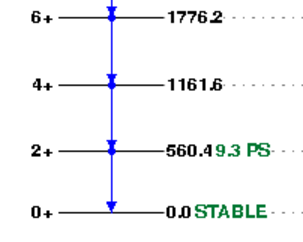
\includegraphics{images/te_120_rot} &
    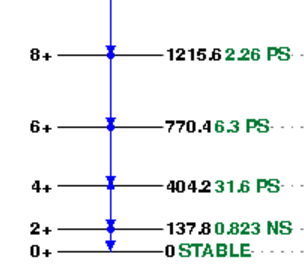
\includegraphics{images/dy_156_vib} \\
      \small{(a)} & \small{(b)}
    \end{tabular}
    \caption{(a) Shows vibrational structure in Te-120. Notice that the $2^+$,
      $4^+$, and $6^+$ states are all evenly spaced. (b) Shows a
      rotational structure in Dy-156. The levels are not evenly
      spaced, but get larger with $I$ (Both images are from www.nndc.bnl.gov).}
    \label{fig:te120}
  \end{figure}

\end{itemize}

\subsection{Rotation}
\begin{itemize}
\item Nuclei with a lot of valence protons and neutrons may statically
  deform. This is seen with promiscuity:
  \begin{equation*}
    P=\frac{N_pN_n}{N_p+N_n}
  \end{equation*}
Where $N_p$ is the number of valence protons, and $N_n$ is the number
of valence neutrons. Valence nucleons are the extra nucleons after the
last large shell. Around P$>$4, you see
deformation.~\cite[Lec. 13-16]{lecture}
\item Generally occurs in the ranges $150 < A < 190$ and $A > 230$.
\item The deformation parameter $\beta$ tells you how much it is
  deformed.~\cite[Lec. 13-16]{lecture}
  \begin{itemize}
  \item $\beta > 0$: Prolate, rotating around the major axis (egg).
  \item $\beta < 0$: Oblate, rotating around the minor axis (pumpkin)
  \end{itemize}
\item The energy of the states is proportional to the $J$ of the
  state, and the moment of inertia ($\Im$).
  \begin{equation*}
    E = \frac{\hbar^2}{2\Im}J(J+1)
  \end{equation*}
Instead of the angular momentum squared, like in classic mechanics, it
is $J(J+1)$ because this is quantum mechanics and that's how it
works. Get over it. The energy for rotation levels is therefore tied
to the angular momentum $J$ of the level.
\begin{table}[hbt]
\centering
\begin{tabular}{llll}
\textbf{Level} & \textbf{E}         & \textbf{$E_\gamma$}     & \textbf{$\Delta{}E_\gamma$} \\
$0^+$          & 0                  &                   &     \\
$2^+$          & $6(\hbar^2/2\Im)$  & $6(\hbar^2/2\Im)$ & $8(\hbar^2/2\Im)$    \\
$4^+$          & $20(\hbar^2/2\Im)$ & $14(\hbar^2/2\Im)$ & $8(\hbar^2/2\Im)$    \\
$6^+$          & $42(\hbar^2/2\Im)$ & $22(\hbar^2/2\Im)$ & $8(\hbar^2/2\Im)$                     \\
$8^+$          & $72(\hbar^2/2\Im)$ & $30(\hbar^2/2\Im)$  &                      \\
               &                    &                    &                     
\end{tabular}
\caption{Rotational energy levels.}
\label{tab:rotation}
\end{table}
The values in Table~\ref{tab:rotation} look confusing but bear with
me. The table shows energy levels (E) based on the
equation above for a bunch of levels in the nucleus. The E values go up faster
than linearly, (6, 20, 42, etc). The next column shows the 
$\gamma$-ray energy that is emitted to go from a given state to the
\textit{next lower state}. Those also go up, but with a constant
slope. This is shown in the final column, where the $\Delta{}E_\gamma$
is shown. This means that you'll see an equally spaced series of
$\gamma$-rays emitted by a rotating nucleus. You can see this in
practice if you calculate out the energy differences in the Dy-156
rotational levels in Figure~\ref{fig:te120}. You'll find that every
level difference is getting larger by about 100 keV every time.
~\cite[Lec 13-16]{lecture}
\item The difference between two energy levels is given by (from the
  homework):
  \begin{equation*}
    \Delta{}E=E_{J^\pi}-E_{(J-1)^\pi}=\frac{\hbar^2J}{\Im}
  \end{equation*}
\item All the energy for the rotational band levels are tied up in the
  rotation. The nucleus does not actually possess any of the energy,
  and it doesn't affect its state. Much like the Earth's rotation
  doesn't affect you. This means that the wave functions between
  rotation states are almost identical, and so there is an enhanced
  probability of $\gamma$-decay between them. Also, the energy from
  rotation will never cause particle emission, because the rotation
  hasn't ``heated up'' the nucleus. It can just ``slow down'' via
  $\gamma$ emission.\cite[Lec. 13-16]{lecture}
\item The ratio of the $4^+$ and $2^+$ states should almost always be
  close to:
  \begin{equation*}
    R_{42}=\frac{E(4^+)}{E(2^+)} \approx 3.3
  \end{equation*}
\item  Deformation also leads to breaking of degenerate $J$
  substates. Just stick with me:
  \begin{itemize}
  \item Every state has an associated $J$ value (for example, a $p_{3/2}$
    state has $J=3/2$).
  \item $(2J+1)$ nucleons can live there because they can have their
    own $m_j$ values that range from $-j \ldots j$, by integer
    values. The energy level has a \textit{degeneracy} of $(2J+1)$. 
    \begin{framed}
    \textbf{Note:} Per Andrew, there won't be anything on the
      Nielsen model on the exam. This is the following few bullets
      about the energy levels splitting in a deformed nucleus.
    \item When the nucleus becomes deformed, this isn't true
      anymore. Now that there is a preferred direction (the axis of
      rotation), nucleons with different values of $m_j$ will split
      out.
    \item The level splits into all of it's different components. The
      $+j$ and $-j$ components have the same energy because the
      nucleus is symmetric.
    \item The energy levels now depend on how long the nucleon spends
      close or far from the nucleus, depending on it's angular
      momentum. See Figure~\ref{fig:levelsplit}.
    \end{framed}
    \begin{figure}[hbt]
      \centering
      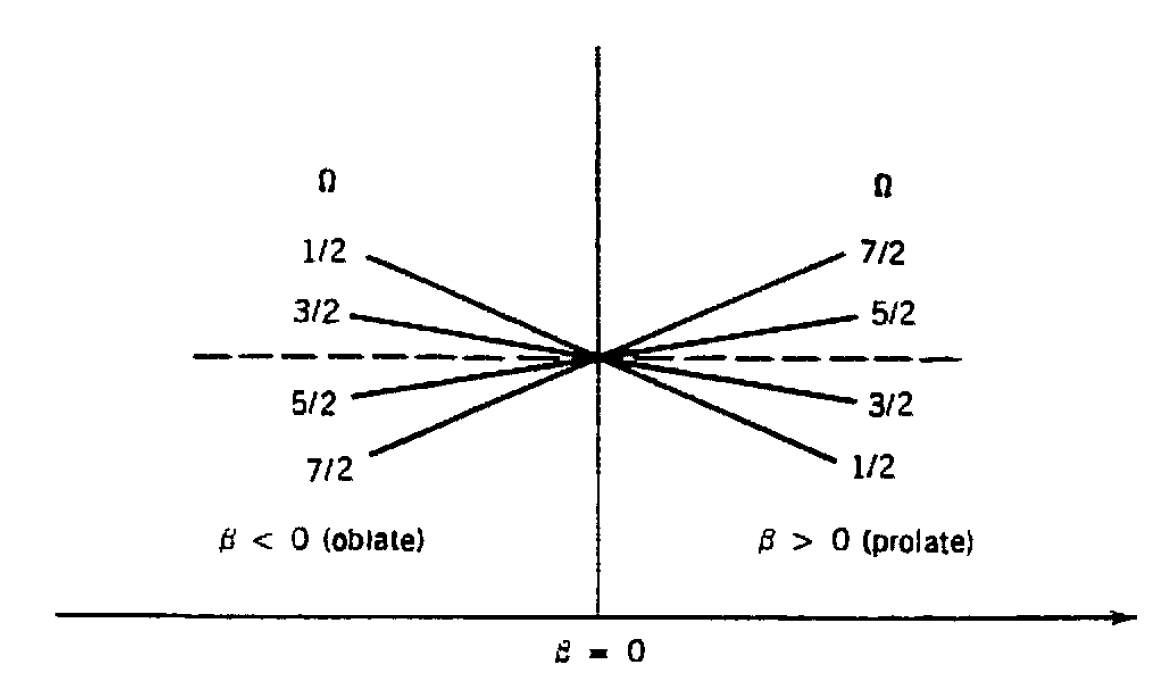
\includegraphics[scale=0.5]{images/levelsplit}
      \caption{Krane Figure 5.27, splitting of the levels of the
        $f_{7/2}$ orbit in a deformed nucleus.\cite[pp. 153]{krane}}
      \label{fig:levelsplit}
    \end{figure}
  \end{itemize}
\cite[pp.151-153]{krane}
\end{itemize}

\section{$\alpha$-decay}

\begin{itemize}
\item The $\alpha$-decay half-life can be estimated using a barrier
  tunneling model. You can calculate the frequency of collision with
  the potential well and use the transmission probability to calculate
  a half-life. This isn't the real model and only represents an
  electromagnetic baseline to give us insight into what is
  happening. It isn't \textit{nuclear}.~\cite[Lec. 18]{lecture}
\item Any angular momentum carried away by the $\alpha$-particle is
  \textbf{purely orbital}. The spins all couple pairwise to
  0. The angular momentum change from $\alpha$-decay can range from:
  \begin{equation*}
    |I_i-I_f| \leq l_{\alpha} \leq I_i + I_f
  \end{equation*}
With parity change:
\begin{equation*}
  \Delta\pi = {(-1)}^{l_{\alpha}}
\end{equation*}
The simplest decay is any $0 \to X$ state, because the only value
for $l_{\alpha}$ is $X$. If that doesn't give the right parity change,
the decay is \textit{forbidden}. In this case it really means
\textit{forbidden}, unlike $\beta$-decay, which plays fast and loose
with the term.~\cite[pp. 257-258]{krane}.
\item $\alpha$-decay can populate many different states. Each one has
  a different $Q$-value (given by the $Q$ value for decay to the
  ground state, minus the excitation
  energy).
  \begin{equation*}
    Q = Q_0 - E_{ex}
  \end{equation*}
Where $Q_0$ is the $Q$ value to the ground state and $E_{ex}$ is the
excitation energy of the excited daughter nucleus.
~\cite[pp. 257-258]{krane}.
\item The $Q$-value also gives you the total energy of the two decay
  fragments:
  \begin{equation*}
    Q=T_{X'}+T_{\alpha}
  \end{equation*}
If the original nucleus $X$ was at rest, you can use conservation of
momentum ($p_{\alpha}=P_{X'}$) to get:
\begin{equation*}
  \begin{split}
    T_{\alpha}&=\frac{Q}{(1+m_{\alpha}/m_{X'})} \\[10pt]
    &=Q(1-4/A) \quad \text{with } A \gg 4
  \end{split}
\end{equation*}
The $\alpha$ particle usually has 98\% of the $Q$ value. The typical
$Q$ value is about 5 MeV.~\cite[pp. 248]{krane}
\item The intensity depends on how similar the initial and final wave
  functions are, and the angular momentum ($l_{\alpha}$). The higher
  the $l_{\alpha}$, the less likely the decay.~\cite[pp. 257-258]{krane}.
\item The hinderence factor (HF) tells us about the similarity between
  the parent and daughter states.:
  \begin{itemize}
  \item $1<H<4$ Favored: $\alpha$-particle is from two low-lying pairs
    of nucleons.
  \item $4<H<10$: favorable overlap between initial and final state.
  \item $10<H<100$: spin projections are parallel. Unfavorable overlap
    between initial and final states.
  \item $100<H<1000$: spin projections are parallel, change in parity.
  \item $H>1000$: spin-flip, change in parity.
  \end{itemize}
Any spin flip $\to$ over 1000. Any parity change $\to$ over
100. Non-favorable overlap $\to$ over 10. See
Table.~\ref{tab:alpha-hinderance}.~\cite[Lec. 18]{lecture}
\begin{table}[hbt]
\centering
\begin{tabular}{llll}
\textbf{H}       & \textbf{Nuclear State Overlap} & \textbf{Parity Change} & \textbf{Spins} \\
\textless10   & Favorable                      & None                   & Parallel       \\
10--100           & Unfavorable                    & None                   & Parallel       \\
100--1000         & Unfavorable                    & Yes                    & Parallel       \\
\textgreater1000 & Unfavorable                    & Yes                    & Spin-flip      \\
                 &                                &                        &               
\end{tabular}
\caption{Summary of $\alpha$-decay hinderance factors.}
\label{tab:alpha-hinderance}
\end{table}
\item $\alpha$-decay spectrum has sharp peaks, each represents a decay
  to different excited states. Higher $E_\alpha$, lower excitation
  energy. The excited states then usually release $\gamma$-ray
  photons.~\cite[pp. 262-264]{krane}
\item In an even-even nucleus, the alpha decay to the ground state is
  usually \textit{very strong}. The $0^+ \to 0^+$ decay is not
  inhibited by differences between the wave functions (they are very
  similar. By the same logic, the decay of odd-$A$ nuclei may be
  \textit{very weak} because the two states may be significantly
  different.~\cite[pp.264]{krane}
\end{itemize}

\section{$\beta$-decay}
\begin{itemize}
\item Energy release distribution is continuous because there are two
  particles emitted so they can share any proportion of the
  energy.~\cite[pp. 273, Lec 19]{krane,lecture}
\item Three kinds:
  \begin{equation*}
    \begin{split}
    \beta^-&: n \to p + e^- + \bar{\nu}_e \\
    \beta^+&: p \to n + e^+ + \nu_e \\
    EC&: p + e^- \to n + \nu_e
  \end{split}
  \end{equation*}
Each has a different energy release:
\begin{equation*}
  \begin{split}
    Q_{\beta^-}&=[m(^AX)-m(^AX')]c^2 \\
    Q_{\beta^+}&=[m(^AX)-m(^AX')-2m_e]c^2\\
    Q_{\epsilon}&=[m(^AX)-m(^AX')]c^2-B_n
  \end{split}
\end{equation*}
For $\beta^-$, the electron masses all cancel when using atomic masses
because $-Zm_e+(Z+1)m_e-m_e=0$, that is the electrons accounted for in
the atomic masses for the original atom, final atom and leftover
electron all cancel. They don't cancel for $\beta^+$ because
$-Zm_e+(Z-1)m_e-m_e=-2m_e$. This means that $\beta^+$ decay has a
threshold energy, because the difference in masses must be larger than
$2m_e$ for the $Q$ to be greater than 0.~\cite[pp. 274-276]{krane}
\item The binding energy can be estimated using:
  \begin{equation*}
    B_n=13.6 eV\frac{Z^2}{n^2}
  \end{equation*}
where n is the principle number for the electron.
\end{itemize}

\subsection{Fermi Theory}
\begin{itemize}
\item There are three things that go into
  determining the spectrum of beta decay energy values:
  \begin{equation*}
    \begin{split}
    N(p) &\propto \text{Statistical factor} * \text{Coulomb Interaction
    (electrodynamic)} * \text{Nuclear Matrix Element} \\
  N(p) &\propto p^2(Q_\beta-T_e)^2*F(Z_d,T_e)*|M_{fi}|^2*S(p,q)
\end{split}
\end{equation*}
These terms are:
\begin{itemize}
\item Statistical factor: related to the number of final states
  accessible. Decays like to happen when there are a lot of final
  states that are open.
\item Fermi function ($F$): the influence of the atomic coulomb
  field. This is the \textbf{electrodynamic} part.
\item Matrix element ($M_{fi}^2*S(p,q)$): This is the \textbf{Nuclear}
  part. It is kind of like the hinderance factors for $\alpha$-decay
  and represents the effect of the initial and final states. The $S$
  function only comes into play in \textbf{forbidden} decays, when the
  electron and neutrino have angular momentum ($l \neq 0$, $s$ and $q$
  are terms for the electron and neutrino angular momenta.
\end{itemize}
\cite[pp.281-282]{krane}.
\item You can plot:
  \begin{equation*}
    (Q-T_e) \propto \sqrt{\frac{N(p)}{p^2F(Z',p)}}
  \end{equation*}
Which \textit{should} give you a straight line (Fermi-Kurie plot) that intersects the
$x$-axis at the $Q$ value. For forbidden decays, the line is
\textbf{not} straight, you have to put that $S(p,q)$ factor in on the
bottom to make it straight. This is the \textit{shape factor}, which
then gives you a straight line.~\cite[pp. 282]{krane}
\item Total decay rate: you can integrate some messy function to get a
  messy function for total decay rate:
  \begin{equation*}
    \lambda = \text{Matrix Element Term} * \int\text{$F$-function and statistical factor}
  \end{equation*}
The full equation is in Krane, page 282. What is important is that the
term outside the $\int$ is the \textbf{nuclear} part, and the integral
is the \textbf{electrodynamic} part. Those are the two things (and
some constants) that determine the decay rate. You can just crunch the
integral and look up values, which is $f$, or the \textit{Fermi
  Integral}. Then, if you do $\frac{f}{\lambda}$ or just $ft_{1/2}$,
then the integrals cancel and all you have is the Matrix Element part,
the \textbf{nuclear} part. This lets us compare $ft_{1/2}$ values,
which are \textit{only dependent on nuclear
  properties}. It might be useful to think about the $ft$ value as just a
\textit{corrected} half-life. Corrected to remove electrodynamic stuff.~\cite[pp. 282-283, Lecs. 19-21]{krane,lecture}.
\item $ft$ values have a huge range ($10^3$ to $10^{20}$) so we use
  log$ft$ instead.
\end{itemize}
\subsection{Allowed Decays}

\begin{itemize}
\item Electron and neutrino are created at the origin ($r=0$), so
  their angular momentum is $l=0$. There are two modes based on spin:
  \begin{itemize}
  \item \textbf{Fermi Decay}: the spins of the neutrino and electron
    are anti-parallel, so total $S=0$.
  \item \textbf{Gamow-Teller Decay:} the spins are parallel, so the
    total $S=1$.
  \end{itemize}
The difference in the nuclear spin parity ($I^\pi$) before and after
the decay will come from the
$l$ and $S$ that the electron and neutrino carry away. So, if you have
Fermi decay ($l=0$ and $S=0$), there can't be any change in the
nuclear spin $\Delta{}I = |I_i-I_t|=0$. If you have Gamow-Teller decay
($l=0$ and $S=1$), you have $\Delta{}I =$ 0 or 1. 
\begin{framed}
  \textbf{TRICKY PART:} You can have $\Delta{}I = 0$ in Gamow-Teller decay because you can
  couple a vector of length 1 onto a vector and end up with the same
  vector magnitude. This \textbf{does not work} if you started with
  $I_i=0$ because you can't add 1 to 0 and get 0. This means that a
  beta decay from $I_i=0$ to $I_f=0$ \textit{must} be Fermi decay.
\end{framed}
Therefore, all allowed decays have:
\begin{equation*}
  \Delta{}I = 0,1 \quad \Delta{}\pi = \text{no}
\end{equation*}
\cite[pp. 289, Lec. 19-21]{krane,lecture}
\item \textbf{Superallowed Decays:} all super-allowed decays are
  allowed decays, but not all allowed decays are super-allowed. All
  that super-allowed means is that the $ft$ value is 3-4. So they are
  just super-likely.
\end{itemize}

\subsection{Forbidden Decays}

\begin{itemize}
\item Any beta-decay that has $l \neq 0$ is \textbf{forbidden}. This
  doesn't mean that it doesn't happen, it just means it's not very
  likely. This is because angular momentum $\vec{l} =
  \vec{r}\bullet\vec{p}$. The radius where the $\beta$-decay is on the
  order of the nuclear radius ($\approx$ 6 fm) which is \textit{super}
  small. The small radius means a small angular momentum, so it's very
  unlikely that $\beta$-decay will occur with $l \neq 0$. But it does,
  rarely.~\cite[Lec. 19-21]{lecture}.
\item The n\textsuperscript{th} forbidden decay will have $l=n$, and both of the
  spin-arrangements (Fermi for $S=0$ and Gamow-Teller for $S=1$)
  described above. Therefore, you can have:
  \begin{equation*}
    \Delta{}I=0,1,2\ldots(l+1) \quad \Delta\pi = (-1)^l
  \end{equation*}
The $\Delta{}I$ goes up to $l+1$ because Gamow-Teller can have the
spin $S=1$ lined up with the angular
momentum.~\cite[pp.291,Lec.19-21]{krane,lecture}
\item $\beta$-decay will occur via the ``lowest'' decay that it
  can. That is, it will use an allowed decay or the lowest nth
  forbidden decay that can accomplish the transition. You have to look
  at \textit{both} parts of the initial and final states, $I$
  \textbf{AND} $\Delta\pi$ to figure out which it is. Also,
  $\beta$-decay tries to populate states the result in the largest
  energy release (it wants to get to the ground state).~\cite[Lec 19-21]{lecture}
\item Based on the description above, as you get higher in the
  forbidden decays, 1st forbidden to 2nd forbidden etc, the decays
  become less likely. See Table~\ref{tab:logft}.~\cite[Lec. 19-21]{lecture}
\begin{table}[hbt]
\centering
\begin{tabular}{lr}
\textbf{Type of $\beta$-decay} & \textbf{Log($ft$)} \\
Superallowed                   & 3.5                \\
Allowed                        & 4-7.5              \\
1st forbidden                  & 6-9                \\
2nd forbidden                  & 10-13              \\
3rd forbidden                  & 14-20              \\
4th forbidden                  & $\approx$ 23
\end{tabular}
\caption{Log($ft$) values for types of $\beta$-decay}
\label{tab:logft}
\end{table}
\end{itemize}

\subsection{Electron Capture}

\begin{itemize}
\item Almost always, the electron is captured from the inner-most $S$
  orbital, and the neutrino emitted is mono-energetic. Auger electrons
  may result from the cascade of electrons as they move down to fill
  the vacancy left by the lower shells.~\cite[Lec. 19-21]{lecture}
\end{itemize}

\subsection{Helicity}

\begin{itemize}
\item Helicity: helicity is just a property that we define based
  on a particles spin and momentum:
  \begin{equation*}
    h=\frac{\vec{s}\bullet\vec{p}}{|\vec{s}\bullet\vec{p}|}
  \end{equation*}
  Neutrinos have specific helicity based on if they are a neutrino or
  anti-neutrino:
  \begin{itemize}
  \item \textbf{ALL} neutrinos ($\nu$) have helicity $h=-1$
  \item \textbf{ALL} anti-neutrinos ($\bar{\nu}$) have helicity $h=+1$
  \item All electrons \textbf{from $\beta$-decay} have helicity
    $h=-\frac{v}{c}$.
  \item All positrons \textbf{from $\beta$-decay} have helicity
    $h=+\frac{v}{c}$.
  \end{itemize}
  Note that the helicity rules for neutrinos are always always true,
  but the ones for electrons/positrons are only true \textit{if the
    electron is from $\beta$-decay}.
\end{itemize}

\section{$\gamma$-decay}

\begin{itemize}
\item $\gamma$-rays are photons generated from the decay between two
  nuclear states. The radiation comes from the electric and magnetic
  fields generated by charge and current in the nucleus. Therefore,
  there can be radiation caused by electric or magnetic
  fields.~\cite[pp.330]{krane}
\item The radiation fields have multipole orders, as before ($L=1$ is
  dipole, $L=2$ is quadrupole, etc). The parity of the radiation
  fields are:
  \begin{equation*}
    \begin{split}
      \pi(ML)&=(-1)^{L+1} \\
      \pi(EL)&=(-1)^{L}
    \end{split}
  \end{equation*}
~\cite[pp.330]{krane}
\item Therefore, for a given ML or EL transition, we can calculate the
  allowable range of angular momentum change between the initial and
  final states:
  \begin{equation*}
    |I_i-I_f| \leq L \leq I_i+I_f \quad \text{(no }L=0\text{)}
  \end{equation*}
  \begin{equation*}
    \begin{split}
      \Delta\pi &= \text{no: even electric, odd magnetic} \\
      \Delta\pi &= \text{yes: odd electric, even magnetic} \\
    \end{split}
  \end{equation*}
There is no ($L=0$) transitions because the monopole moment is just
the electric field, which does not vary with time. Therefore, the \textit{E}0
and \textit{M}0 transitions are not possible \textit{by the emission
  of a single photon} (it is possible with internal conversion).~\cite[pp. 334]{krane}
\item The lowest $L$-value transition is usually the most probable,
  raising the value of $L$ by one makes the next transition on the order of
  $10^5$ times less probable. Electric transitions are about 100 times
  more likely than magnetic transitions.~\cite[pp. 335]{krane}
\item Weiskoff estimates: using the model in which a single particle
  releases a single photon, we can calculate decay rates. These may be
  \textit{way} off because the state that is decaying may be some
  collective motion of all the nucleons. Therefore, the standing wave
  that is holding the energy of the state may constructively interfere
  and release a $\gamma$ much faster than the estimate would say. Or,
  it could slow down the decay if it adds destructively.~\cite[Lec. 22]{lecture}
\end{itemize}

\subsection{Internal Conversion}

\begin{itemize}
\item An electromagnetic process that occurs with $\gamma$-decay, and
  ``competes'' to be mechanism for decay. The nucleus does not emit a
  photon, but the fields eject an electron from the
  nucleus. This creates peaks on the $\beta^-$ energy spectrum
  (because it's releasing electrons at finite energies).~\cite[pp. 341]{lecture}
\item If the $\Delta{}J$ is large, internal conversion
  becomes much more probable compared to $\gamma$-decay, because a
  $\gamma$-decay with such high $L$ is very rare. It is also more
  probable if the $\Delta{}E$ between the states is close to x-ray
  energy (10-100 keV). It gets much less probable when the energy gets
  higher (5 MeV).
\item The total decay probability is due in some part to the regular
  $\gamma$-decay, as well as the internal conversion (multiple holes
  in the same bucket). We define a ratio of decay probabilities $\alpha$:
  \begin{equation*}
    \alpha = \frac{\lambda_e}{\lambda_\gamma}
  \end{equation*}
It is more useful in this form:
\begin{equation*}
  \lambda_t = \lambda_\gamma(1+\alpha)
\end{equation*}
The $\alpha$ can be split up into specific values for each shell,
$\alpha_K$, $\alpha_L$, $\alpha_M$, etc. In that case you just add
them all up to get the total $\alpha$.
\end{itemize}

\section{Reactions}

\begin{itemize}
\item The reaction:
  \begin{equation*}
    a + X \to Y + b
  \end{equation*}
Can be written in reaction notation as:
\begin{equation*}
  X(a,b)Y
\end{equation*}
\cite[pp. 378-379]{krane}
\item A microscopic cross section ($\sigma$) represents the ``relative
  probability for the reaction to occur.'' It can be used in the
  following equation:
  \begin{equation*}
    R = (\rho{}d)_{target}\times{}I_{beam}\times\sigma_{reaction}
  \end{equation*}
Where $R$ is the reaction rate (in reactions/sec); $(\rho{}d)$ is the
density (in g/cm$^3$) times the width of the target (in cm), also
known as the areal density; $I_{beam}$ is the incident particle flux
(in atoms/sec); and $\sigma_{reaction}$ is the microscopic cross
section of the reaction occurring. This is only valid when very little
of the beam reacts (small $\sigma$) and everything moves in straight
lines.~\cite[Lec. 25]{lecture}
\item Microscopic cross sections are generally given in units of
  barns. 1 barn = $10^{-24}$ cm$^2$.
  \item The cross section is not always constant over angle (it rarely
    is). So the \textit{differential cross section} is used:
    \begin{equation*}
      \frac{d\sigma}{d\Omega}
    \end{equation*}
    What is confusing, is this is just
    a number, in units of barns/steradian. It's
    representing the fact that some small number of particles
    ($d\sigma$) will strike our small detector ($d\Omega$). It is
    dependent on the angle of scatter ($\theta$) and the polraization
    of the radiation ($\phi$). Generally we assume there is no affect
    due to polarization (things are randomly polarized).

We can
    find the size of our detector $d\Omega$ in steradians, which is
    related to the area of our detector ($dA$) and the distance from
    the target ($r$) by:
    \begin{equation*}
      d\Omega = \frac{dA}{r^2}
    \end{equation*}
    Then, if we know the differential cross section at the angle of
    our detector, we can multiply to get the reaction cross section
    for our detector:
    \begin{equation*}
      \sigma_{det} = d\Omega\frac{d\sigma}{d\Omega}
    \end{equation*}
    This represents something \textbf{very specific}. This is the
    probability that incoming particles striking the target will then
    be detected by our detector. Based on the size of our detector
    ($d\Omega$) and our a priori knowledge of the number of particles
    that will be seen in a small area ($\frac{d\sigma}{d\Omega}$). The
    value of that differential cross section will probably vary with
    angle, so you have to know the differential cross section for the
    angle where your detector is to even use this. More rigorously,
    you'd integrate over the area of the detector and
    $\frac{d\sigma}{d\Omega}$ may vary over the integral:
    \begin{equation*}
      \sigma_{det} = \int_{detector}\frac{d\sigma}{d\Omega}d\Omega
    \end{equation*}
    Or, you can get the total $\sigma$ by integrating over the whole
    angle space.
\item \textbf{Rutherford Differential Scattering:} elastic Coulomb
  scattering. An incoming particle scatters off the potential of the
  target.~\cite[Lec 24]{lecture}
\item \textbf{Coulomb Excitation:} inelastic Coulomb scattering. An
  incoming particle scatters off the potential of a target and leaves
  some energy behind. This ``Coulex'' reaction can excite nuclei up
  rotational bands.~\cite[Lec. 24]{lecture}
\end{itemize}

\bibliographystyle{unsrt}
\bibliography{NE101}
\end{document}
